\chapter{Tools for Neuromechanical Simulation}\label{ch:sns}
\graphicspath{{../Figures/60-sns/}{figs/60-sns/}}

This chapter follows the development of tools for transferring neural controllers between mechanical models. An initial AnimatLab walker motivated the move to Gait2392, graphical neural construction, and accelerated simulation. These capabilities were then combined with staged controller training and BPA-actuated robot models.

\section{Motivation: The AnimatLab Story}\label{sec:prior_walker}\label{sec:animatlab_results}

For a course project in ME 610: Neuromechanical Modeling, Morrow and I coupled the bipedal mechanics of \citet{li_bipedal_2017} with the two-level central pattern generator (CPG) of \citet{deng_neuromechanical_2019} in AnimatLab \citep{cofer_animatlab_2010}. The model had bilateral thigh, shank, foot, and toe segments, sagittal-plane joints, and antagonist Hill-type muscles at the hip, knee, and ankle. I added a passive toe joint. A shared rhythm generator (RG) supplied bilateral pattern-formation (PF) and motor-neuron (MN) pathways, with afferent feedback at the MN level. We adjusted currents, synaptic weights, and muscle parameters by hand and presented the suspended stepping result at the 2021 NIH BRAIN Initiative Investigators Meeting \citep{bolenTorqueValuesArtificialKnee2021June15-17}.

In a saved graded-neuron trial, alternating activity propagated through the RG, PF, and MN layers while the hip, knee, and ankle cycled at approximately \qty{2.2}{\hertz}. The aligned recording is retained in Appendix~\ref{app:simulation_verification} (Figure~\ref{fig:animatlab_short_response}). When released toward the ground, the model lost support while the neural rhythm continued (Figure~\ref{fig:animatlab_model_architecture}). The controller schematic is shown separately in Figure~\ref{fig:animatlab_shared_rg}. This contrast between suspended motion and ground loading motivated a workflow for retuning a circuit when its mechanics and sensory conditions change.

\begin{figure}[htbp]
\centering
\begin{minipage}[c]{0.46\textwidth}\centering
\textbf{(A)}\\[2pt]
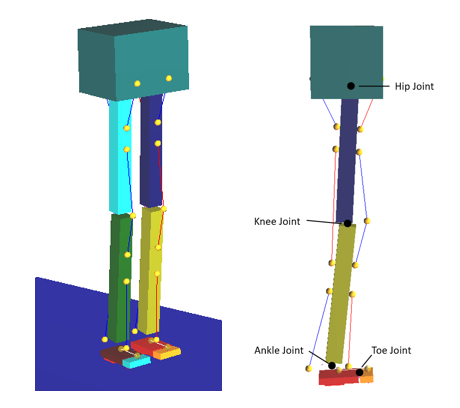
\includegraphics[width=\linewidth,height=0.19\textheight,keepaspectratio]{OurWalker.png}
\end{minipage}\hfill
\begin{minipage}[c]{0.46\textwidth}\centering
\textbf{(B)}\\[2pt]
\includegraphics[width=\linewidth,height=0.19\textheight,keepaspectratio]{LI_DENG_FALL_FRAME.png}
\end{minipage}
\caption[Original AnimatLab walker and ground-test fall]{\textbf{(A)} Original AnimatLab walker developed by Morrow and Bolen. \textbf{(B)} The model tipping during the ground test.}
\label{fig:animatlab_model_architecture}
\end{figure}

\section{Knowledge Gap and Framing}\label{sec:sns_gaps}

The central problem was how to transfer an identifiable neural controller to a different mechanical model and train it efficiently. Changing muscle geometry, joint motion, inertia, or actuator type changes both the force produced by a neural command and the sensory signals returned to the circuit. The target was a detailed Gait2392 human model, followed by a robot counterpart actuated by BPAs. Comparing controllers therefore required consistent command and sensory interfaces, explicit mechanical checks, and repeatable training conditions.

I developed a workflow that combines graphical circuit construction with automated experiments. OpenSim and MyoConverter supply musculoskeletal mechanics, SNS-Toolbox supplies neural formulations, and Simulink/Simscape supplies graphical neural and mechanical modeling \citep{delp_opensim_2007,caggiano_myosuite_2022,todorov_mujoco_2012,nourse_sns_2023}. My contributions are the model implementations, custom blocks, actuator interfaces, and experiment drivers that connect these tools. The following sections build these capabilities around the Gait2392 reference before combining them in the supported robot example.

\begin{sidewaysfigure}[p]
\centering
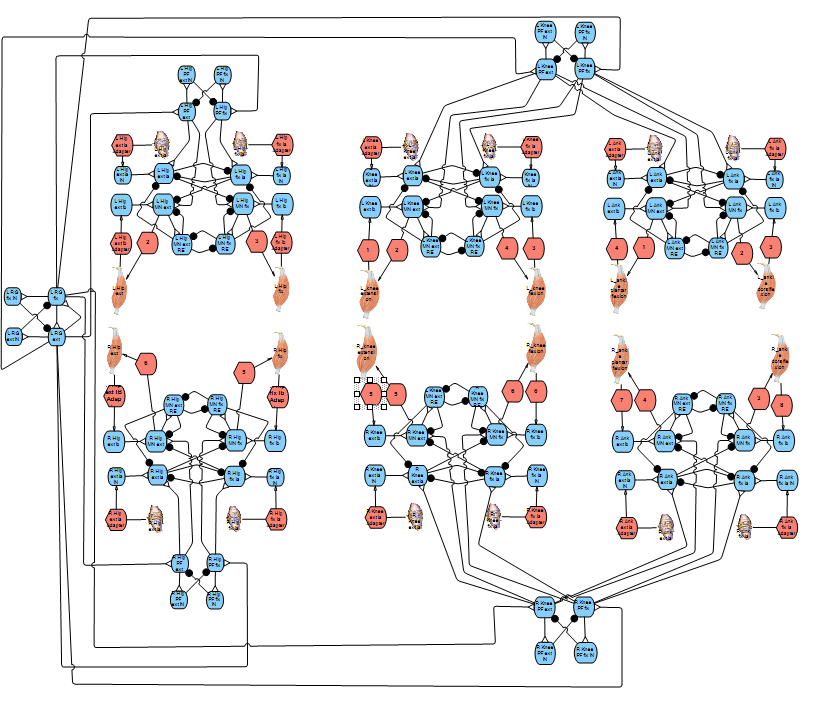
\includegraphics[width=\textheight,height=0.87\textwidth,keepaspectratio]{connor_ben_shared_rg_original.png}
\caption[Original shared-RG controller]{Original shared-rhythm-generator controller. The four-neuron RG supplies bilateral hip and knee/ankle pattern-formation groups.}
\label{fig:animatlab_shared_rg}
\end{sidewaysfigure}

\section{Gait2392 and Controller Transfer}\label{sec:sns_existing_tools}\label{sec:sns_gait_comparison_main}

I converted the Gait2392 human reference from OpenSim to MuJoCo with MyoConverter and connected it to SNS-Toolbox. The robot counterpart required separate treatment: its BPA paths could not simply be combined with unchanged human-muscle parameters. I therefore retained biological-muscle actuators in the human reference and implemented routed BPA forces for the robot counterpart.


\begin{figure}[htbp]
\centering
\includegraphics[height=0.30\textheight]{Gait2392_human_reference_oblique.png}
\caption[Converted Gait2392 human geometry and muscle paths]{Converted Gait2392 human reference with bilateral muscle routes in a static flexed-knee pose. The geometry supports the neural-controller and actuator comparisons; this view is separate from the CAD-derived robot assembly.}
\label{fig:gait2392_human_geometry}
\end{figure}

The converted human model retains 92 actuator entries. Six small hip-rotator entries, the quadratus femoris, gemelli, and piriformis on each side, are disabled and contribute no force. The knee retains OpenSim's flexion-negative convention. Before interpreting a controller's motion, I checked muscle attachments, joint-action directions, force scale, and intended foot contact. Appendix~\ref{sec:app_conversion_repairs} records the conversion repairs and force comparison. Neural and mechanical signals are exchanged at a \qty{2}{\milli\second} solver time step.

For artificial-muscle simulations, I implemented an actuator-force calculation that evaluates the quasi-static BPA model from Chapter~\ref{ch:muscles} at the current simulated actuator length and commanded pressure. The calculated tensile force acts along the model's specified tendon route. Length, velocity, force, and foot-contact measurements are then returned to the neural controller through sensory channels. This closes the neural-command--actuator-force--sensory-feedback loop. The calculation represents the measured static force dependence; it does not add valve-flow or pressure-transient dynamics. Routing geometry and dynamic actuator loading therefore require their own checks beyond the isometric force fit.

The SADb of Chapter~\ref{ch:database} supplies the physiological context for selecting Ia, II, Ib, and contact pathways. A database link identifies the supporting observation; it does not by itself determine a numerical gain or guarantee the same function in another model. The implemented encoding, connection sign, phase gating, and tested response therefore remain explicit parts of the controller specification.

Table~\ref{tab:sns_model_configurations} distinguishes the model bodies, actuation, and representative tests. A controller organization, such as the W2L layout, can be applied to more than one body; its name does not identify the mechanical model. Figure~\ref{fig:mujoco_model_views} contrasts the converted Gait2392 robot with the reduced-order knee model used for block demonstrations.



Single-actuator and matched-pose tests checked the converted mechanics before closed-loop controller tests. These checks separated conversion faults from changes caused by neural control.

At matched poses and OpenSim static-optimization activations (Figure~\ref{fig:force-compare}; Table~\ref{tab:force-r2}), eight of twelve sampled muscles had force-prediction $R^2$ between 0.87 and 0.98 and mean forces within \qty{10}{\percent} of the reference. Rectus femoris and biceps femoris short head had negative $R^2$, indicating errors greater than a constant mean-force prediction. This comparison checks force predictions in the repaired MyoConverter-derived human model while identifying remaining muscle-specific differences. Because the comparison sets pose and activation frame by frame without reproducing trajectory velocities or tendon dynamics, it does not establish dynamic equivalence between the muscle formulations. That distinction matters when interpreting feedback based on muscle force.

These controller comparisons use a common mechanical reference and the same sensory and recording interfaces. Pathway removal tests how a controller uses feedback, while inverse-kinematics overlays show the resulting joint timing and amplitude relative to human motion. Appendix~\ref{sec:gait_library_results} retains the controller comparisons, and Appendix~\ref{sec:app_ik_overlay} retains the direct trajectory comparison. The next requirement was to make these experiments practical both through graphical circuit editing and through automated simulation.

\FloatBarrier

\section{Building the Neuromechanical Simulation Workflow}\label{sec:preliminary_sim_methods}\label{sec:preliminary_sim_results}

The Gait2392 reference defines the detailed mechanical target. The workflow also retains the simpler W2L model as a test case for checking circuit calculations, sensory pathways, and controlled perturbations before interpreting full-body results. Table~\ref{tab:sns_capability} summarizes the capabilities, and Table~\ref{tab:sns_model_configurations} distinguishes controller organization from mechanical body and actuator type.

Graphical blocks support circuit construction, subnetwork inspection, and interactive stimulus application. Headless execution runs the same experiment without opening its graphical interface, allowing parameter searches and repeated perturbation tests to be automated. An application programming interface (API) exposes commands for constructing, controlling, and recording experiments; a software development kit (SDK) supplies supporting libraries and tools. Saved configurations and traces connect these automated runs to graphical review.

\begin{table}[htbp]
\centering
\caption[Models and tools developed for neuromechanical experiments]{Models and tools developed for neuromechanical experiments.}
\label{tab:sns_capability}
\small
\begin{tabularx}{\textwidth}{@{}>{\raggedright\arraybackslash}p{0.28\textwidth}>{\raggedright\arraybackslash}X@{}}
\toprule
\textbf{Model or tool} & \textbf{What it is used for} \\
\midrule
Li--Deng/W2L walker and controller & Combine walker mechanics and neural control in AnimatLab and MuJoCo with SNS-Toolbox; compare matched implementations of the contact-driven neural core in NumPy and Simulink. \\
Gait2392-based models & Compare alternative neural controllers on the human reference model and a robot counterpart with BPA routing and the force model from Chapter~\ref{ch:muscles}. \\
SNS-Simscape block library and editor & Build neural pathways graphically from sensory, neuron, synapse, activation, and muscle-force blocks, including custom BPA blocks. \\
SOLIDWORKS-derived robot assembly & Couple a CAD-derived Simscape Multibody mechanism to a neural controller and BPA actuators using the force model. \\
MuJoCo--Simulink integration & Run an SNS-Simscape controller with a MuJoCo mechanical model through the MathWorks bridge, exchanging actuator commands and sensory measurements. \\
Curriculum and experiment drivers & Tune controllers in stages, vary support and sensory pathways, apply neural stimuli or mechanical perturbations, and record neural and mechanical responses. \\
Literature circuits and spiking variants & Compare selected published neural mechanisms and the behavior of graded and spiking implementations. \\
Accelerated execution and actuator options & Run neural and muscle calculations with compiled kernels, compare execution time, and select biological-muscle, compliant-tendon, or BPA force implementations. \\
\bottomrule
\end{tabularx}
\end{table}

\begin{table}[htbp]
\centering\small
\caption[Neuromechanical models and representative tests]{Model bodies, actuator formulations, support conditions, and representative evaluations.}
\label{tab:sns_model_configurations}
\begingroup
\renewcommand{\arraystretch}{1.15}
\begin{tabularx}{\textwidth}{@{}>{\raggedright\arraybackslash}p{0.21\textwidth}>{\raggedright\arraybackslash}p{0.25\textwidth}>{\raggedright\arraybackslash}p{0.17\textwidth}>{\raggedright\arraybackslash}X@{}}
\toprule
\textbf{Mechanical model} & \textbf{Controller and actuation} & \textbf{Support} & \textbf{Representative evidence} \\
\midrule
Gait2392 human & Alternative graded or spiking SNS; biological muscles & Virtual harness in ground tests; suspension in air tests & Reference-trajectory overlays and pathway-removal comparisons \\
\addlinespace[6pt]
Gait2392 robot counterpart & SNS; routed BPA force model & Test-specific virtual support & Artificial-muscle force and sensory-signal interfaces \\
\addlinespace[6pt]
Li--Deng/W2L walker & Two-level controller; source-model muscle interfaces & Suspension or virtual-walker support & Air stepping, implementation agreement, and feedback tests \\
\addlinespace[6pt]
CAD robot in Simscape & SNS-Simscape; BPA model & Virtual harness & Integrated standing example \\
\addlinespace[6pt]
CAD robot in MuJoCo & Neural timing and force allocator; reference-tension actuators & Specified mechanical assistance & Supported stance and abductor-control comparison \\
\addlinespace[6pt]
\bottomrule
\end{tabularx}
\endgroup
\end{table}

Figure~\ref{fig:simulation_workflow} shows how the model-construction routes and controller interfaces connect. Chapter~\ref{ch:overall} places them within the broader simulation-to-hardware workflow (Figure~\ref{fig:pipeline}). Detailed configurations and evaluation sets are retained in Appendix~\ref{app:simulation_verification}.

\begin{figure}[htbp]
\centering
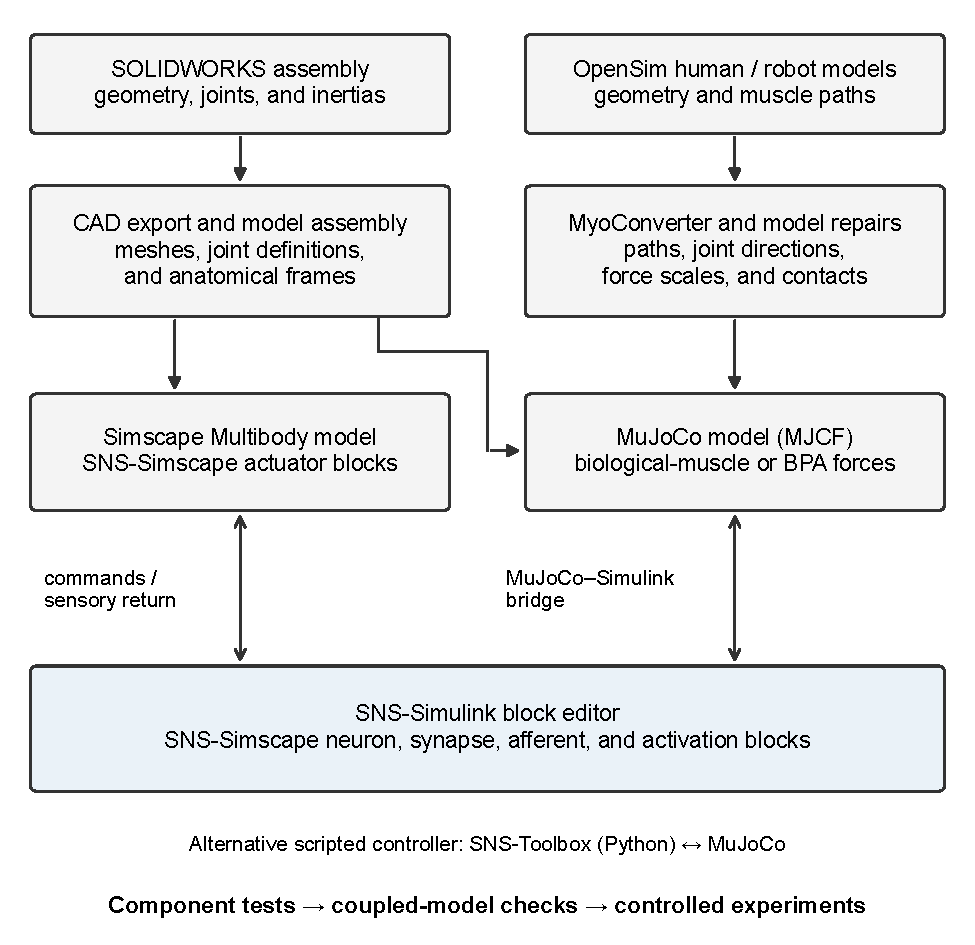
\includegraphics[width=\textwidth,height=0.72\textheight,keepaspectratio]{simulation_workflow.pdf}
\caption[Model construction and neural-controller interfaces]{Model construction and neural-controller interfaces. SOLIDWORKS-derived geometry supplies Simscape Multibody and separately assembled MuJoCo models; OpenSim models follow the MyoConverter and repair route. The SNS-Simulink block editor assembles controllers from SNS-Simscape library blocks. Commands and sensory measurements couple these controllers to Simscape or, through the MuJoCo--Simulink bridge, to MuJoCo. }
\label{fig:simulation_workflow}
\end{figure}

\subsection{Li--Deng/W2L Walker and Controller}\label{sec:sns_w2l_methods}
I replaced the original shared RG with one RG on each side, linked through commissural pathways. The bilateral PF and MN organization was retained, while afferent feedback was extended to the RG and PF layers and heel- and toe-contact channels were added. This later controller is referred to as Walker Two-Layer (W2L).

The newer bilateral W2L implementation contains 108 graded neurons and 216 chemical connections. Separate type-II relays serve flexor and extensor muscles at both hips, knees, and ankles, alongside retained phase-related feedback and distinct heel/toe contact channels. Figure~\ref{fig:w2l108_subnetworks} illustrates the selected left RG and hip organization from the bilateral W2L reference drawing. The aligned stimulus recordings in Appendix~\ref{sec:app_layer_stimulus} connect this circuitry to joint motion.

\begin{figure}[p]
\centering
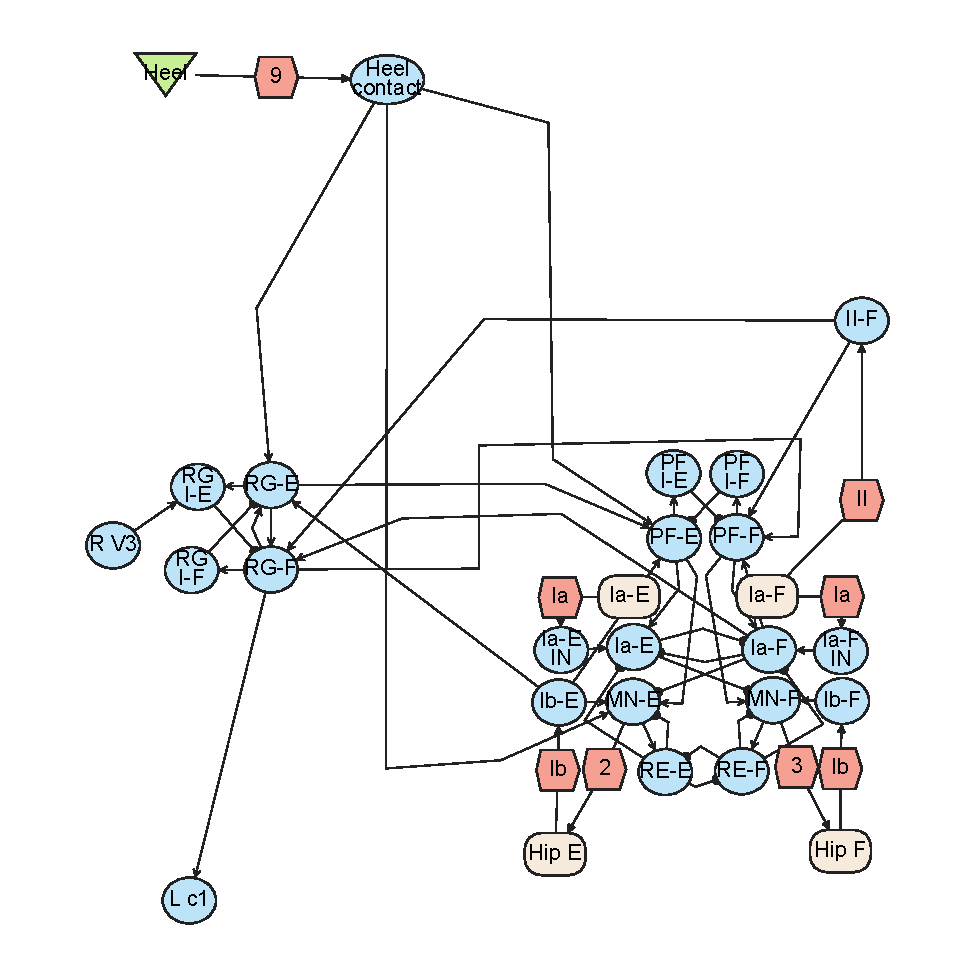
\includegraphics[width=0.8\textwidth]{w2l_selected_left_subnetwork.pdf}
\caption[Selected left W2L rhythm and hip subnetwork]{Selected left RG and hip subnetwork of the bilateral W2L reference. Connections leaving the selection are omitted. Muscle and spindle images are replaced with labeled vector symbols. E/F denote extensor/flexor; Ia, II, and Ib identify sensory pathways, and RE denotes Renshaw interneurons.}
\label{fig:w2l108_subnetworks}
\end{figure}
\label{sec:crossengine_results}\label{sec:sns_feedback_test}

For cross-implementation checks of the contact-driven W2L rhythm core, I used the same neuron definitions, synaptic connections, and parameter values, with identical drive and contact inputs in NumPy and Simulink. Closed-loop experiments held a saved controller fixed while changing selected sensory pathways, drive, or support. Appendix~\ref{app:connectomes} documents the bilateral pathways and conductances of the independently replayed W2L configuration.

Under these matched inputs, burst periods matched at \qty{1.000}{\second}, all ten expected bursts were reproduced, and voltage-trace correlation was at least 0.99996 (Figure~\ref{fig:w2l_crossengine}). This matched-input comparison verifies the rhythm-core implementation.

Removing the phasic heel-contact inputs caused the circuit to latch in both implementations. The alternating activity therefore depends on the specified sensory drive.

\begin{samepage}
The saved W2L controller was tested with all saved effective gains delivered to the compiled network. With controller, drive, and support settings fixed, disabling all sensory feedback shifted median bilateral contact phase from 0.498 to 0.223 cycles. A phase of 0.5 cycles indicates alternating foot loading; the supported-stepping criterion accepts 0.35--0.65 cycles. Forward progression and joint cycling persisted, but the feedback-disabled condition failed this criterion for supported stepping (Figure~\ref{fig:sns_ablation_pair}). Over the \qtyrange{4.5}{30}{\second} scored window, forward displacement was \qty{2.239}{\meter} with feedback and \qty{1.996}{\meter} without it. The comparison identifies a sensory-feedback contribution to bilateral contact coordination. Additional pathway deletions and stimulus tests are summarized in Appendix~\ref{sec:app_w2l_perturbations} (Figure~\ref{fig:app_w2l_perturbations}).\par
\end{samepage}



\begin{figure}[t]
\centering
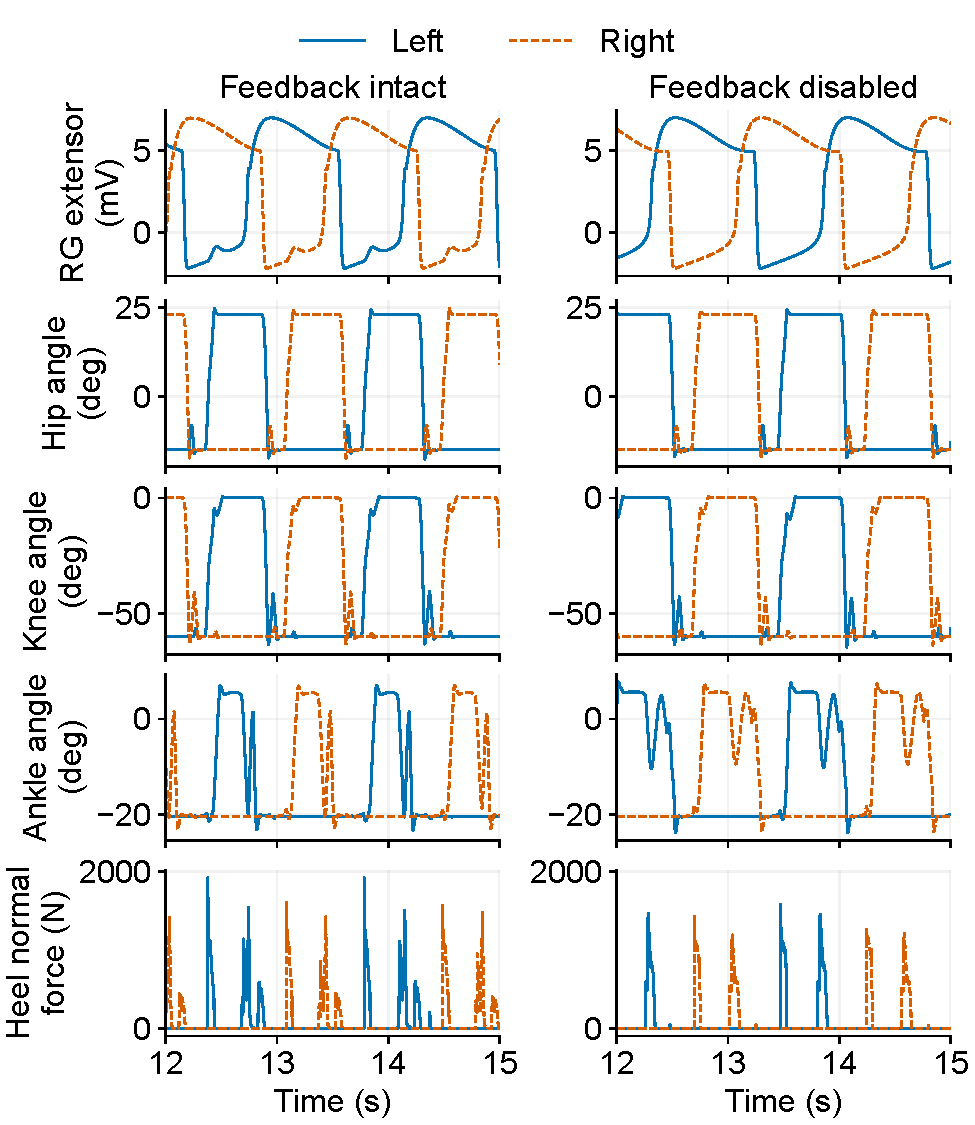
\includegraphics[width=\textwidth,height=0.74\textheight,keepaspectratio]{w2l_feedback_short_20261031.pdf}
\caption[Sensory-feedback comparison in the recovered W2L model]{Sensory-feedback comparison with fixed W2L conductances, drive, and support settings. Extensor-RG voltages, hip, knee, and ankle angles, and heel normal forces are shown over the same \qtyrange{12}{15}{\second} interval, with feedback intact (left) and all sensory feedback disabled (right). Blue solid and orange dashed curves denote the left and right legs. Cycling persists in both conditions. Over the full scored window, median bilateral contact phases are 0.498 and 0.223 cycles; the latter falls outside the 0.35--0.65 acceptance interval.}
\label{fig:sns_ablation_pair}
\end{figure}

Anatomical action checks, initial-pose alignment, and bilateral recruitment adjustments produced nine left and eight right qualifying swings over ten seconds in the newer supported MuJoCo implementation (Figure~\ref{fig:walker_fall_to_supported}). Passive rails and guides retained controllable support while the legs alternated.

\begin{figure}[htbp]
\centering
\includegraphics[width=0.55\textwidth,height=0.23\textheight,keepaspectratio]{W2LNEW_TREADMILL_STILL.png}
\caption[Supported W2L treadmill stepping]{Newer W2L model stepping on the MuJoCo treadmill with passive rails and guides; mean net assistance is 40.5\% of body weight.}
\label{fig:walker_fall_to_supported}
\end{figure}

These controlled comparisons establish a reusable test case. To construct and alter the same kinds of neural pathways graphically, I next developed the SNS-Simscape blocks and editor.

\FloatBarrier

\subsection{SNS-Simscape Block Library and Editor}\label{sec:sns_new_tools}\label{sec:sns_simulink_demos}

\label{sec:w2l_matlab_attempt}

I used MATLAB for graphical controller experiments, using Simulink for the neural controller and Simscape Multibody for the mechanical model. Motor-neuron outputs passed through activation and muscle-force blocks to act on the mechanical model; muscle and joint measurements returned through afferent-encoder blocks as sensory input. Importing a mechanism and obtaining neural oscillation separately checked individual components. Testing the closed loop was also necessary because the timing, magnitude, and sign of those exchanged signals determine the coupled response.

The MATLAB work included both mechanical-model import and neural-response comparisons, followed by coupled simulations. Selected neural implementations reproduced their reference responses, and mechanical import provided models that could be assembled and simulated. Longer comparisons identified useful calibration targets: a full-network export agreed with its reference during an early transient and subsequently diverged, while one constant-drive Simulink realization reached a steady state and its NumPy reference oscillated (Appendix~\ref{sec:sns_ports}). These checks guided separate verification of neural dynamics, actuator action, and sensory coupling before full-model tests.

I subsequently developed both block-programmed and scripted implementations, allowing controller experiments through SNS-Simscape or MuJoCo with SNS-Toolbox.

The SNS-Simscape library implements neuron, synapse, afferent-encoder, activation, and muscle-force elements as editable Simulink blocks. The library retains the conductance-based neuron and synapse formulation supplied by SNS-Toolbox; it does not introduce a new neuron model. Verification uses selected circuits under matched inputs. Figure~\ref{fig:simulink_sns_implementation} shows the core blocks and graded-neuron signal flow.

I used reduced-order reflex demonstrations to check the graphical blocks in a coupled model before assembling a full locomotor controller. In these examples, the sensory pathway, neural response, and mechanical correction can be inspected directly.

The library assembles Ia stretch excitation, reciprocal inhibition, and Ib autogenic inhibition in a reduced-order antagonist knee model (Figure~\ref{fig:sns_reflex_current}\textbf{(C)}). After the model reaches a steady operating point, a \qty{2}{\nano\ampere}, \qty{30}{\milli\second} current pulse at the extensor Ia sensory-neuron input evokes \ang{1.09} of extension, peaking \qty{111}{\milli\second} after pulse onset. The knee then returns toward the matched no-stimulus trajectory, meeting the specified recovery thresholds after \qty{6.355}{\second}. The displayed configuration broadens the MN and Ia synaptic saturation ramps; the original narrow-ramp settings maintained oscillations. This is a transient test of the implemented feedback and actuator equations, rather than a physiologically calibrated tendon-tap model. Appendix~\ref{sec:app_knee_transient} gives the configuration and numerical checks, with the complete response in Figure~\ref{fig:app_knee_transient}.

\begin{samepage}
A second demonstration tests feedback in an arm holding a beverage container as it is loaded (Figure~\ref{fig:sns_beverage_current}). With the reflex enabled, arm sag was \ang{2.00}, compared with \ang{7.85} when it was disabled. As the forearm sags, biceps stretch feedback excites the biceps motoneuron and reciprocally inhibits the triceps motoneuron. The separate Ib pathways provide autogenic inhibition of each muscle. The reduced sag demonstrates a corrective effect of the implemented sensory pathways in the coupled neural and actuator blocks.\par
\end{samepage}

\begin{figure}[p]
\centering
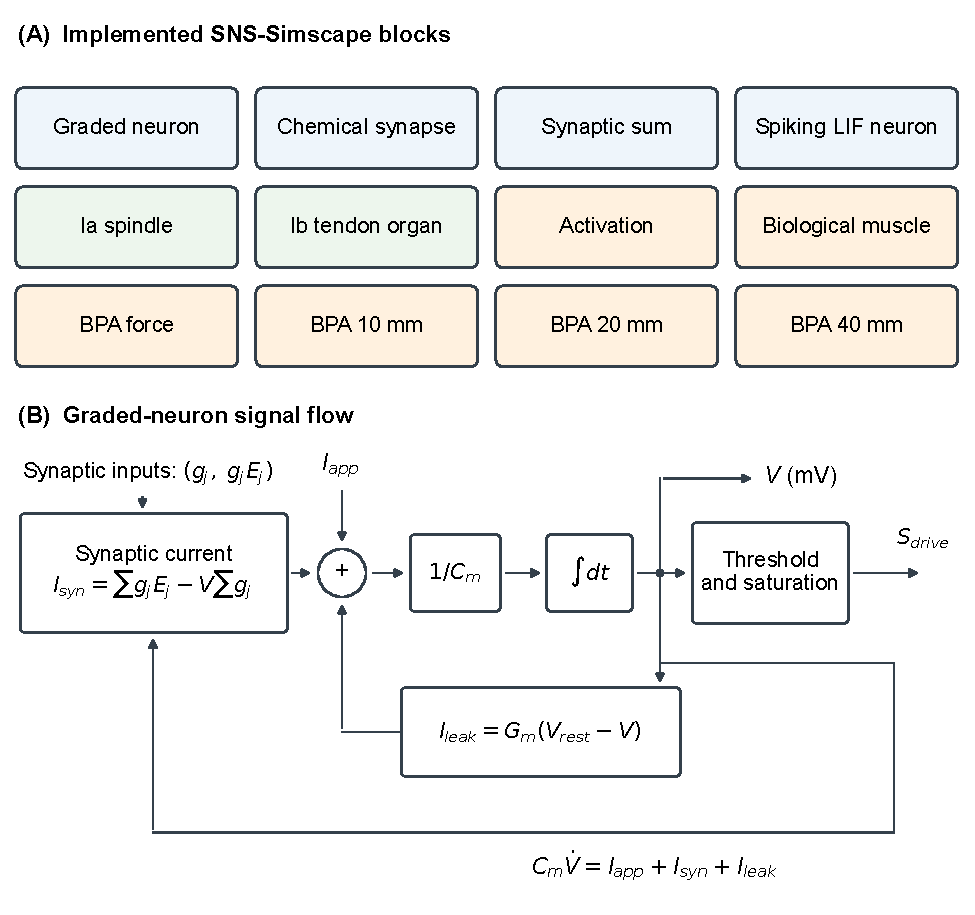
\includegraphics[width=\textwidth,height=0.84\textheight,keepaspectratio]{sns_library_clean.pdf}
\caption[Editable SNS blocks and gradFed-neuron signal flow]{\textbf{(A)} The twelve implemented SNS-Simscape library elements, redrawn as a functional block catalog. \textbf{(B)} Signal flow of the implemented graded neuron: synaptic conductance and reversal-potential products form the synaptic current, which is combined with applied and leak currents before membrane integration. Membrane voltage and normalized drive are separate outputs.}
\label{fig:simulink_sns_implementation}
\end{figure}

\begin{figure}[p]
\centering
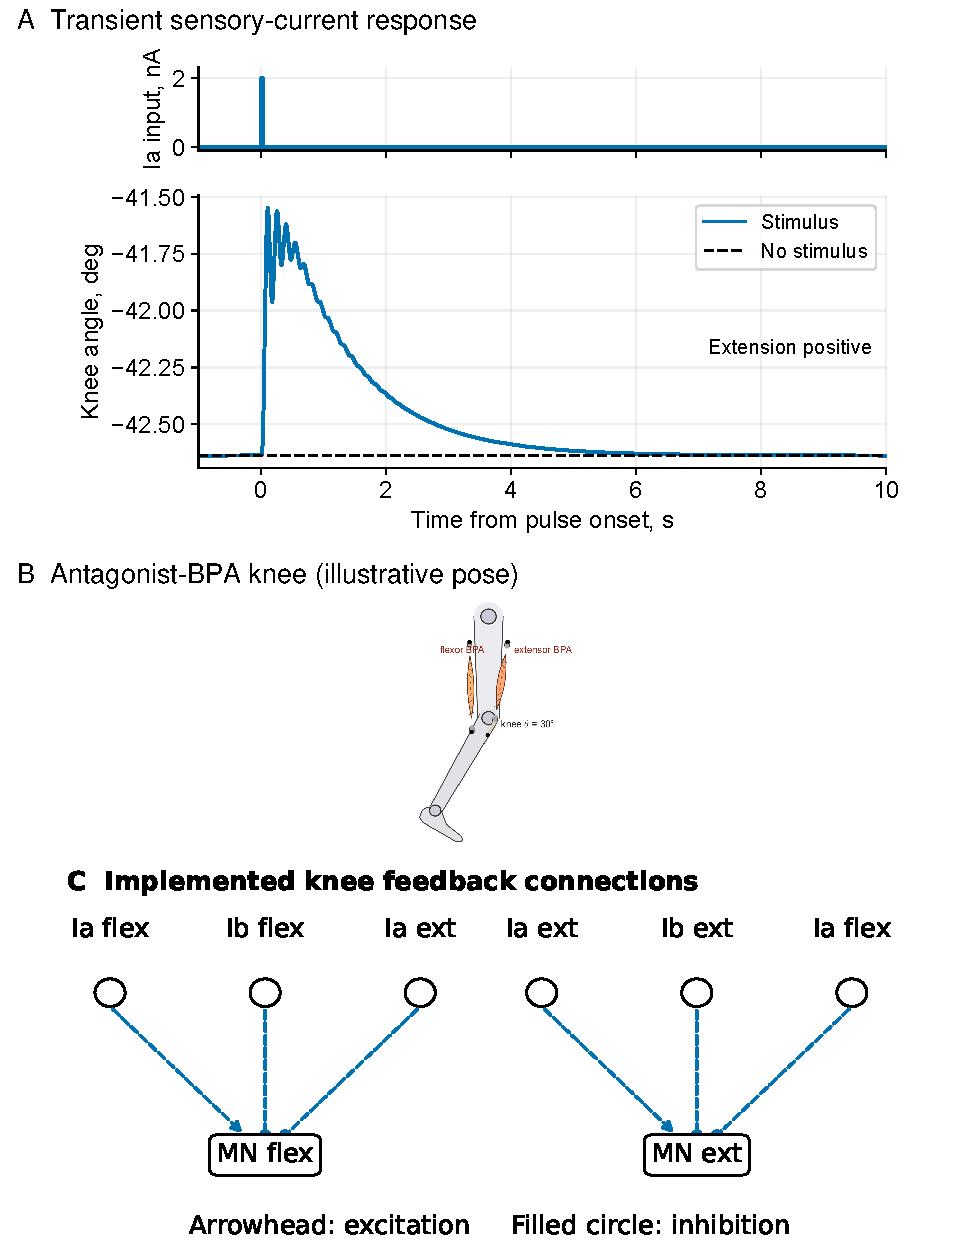
\includegraphics[width=\textwidth,height=0.80\textheight,keepaspectratio]{knee_transient_current_layout.pdf}
\caption{Transient knee response to a \qty{2}{\nano\ampere}, \qty{30}{\milli\second} sensory-current pulse after settling (A), antagonist-BPA leg schematic in an illustrative pose (B), and the six implemented feedback connections (C). Flexion is negative. The graded-response configuration uses broadened MN and Ia synaptic saturation ramps; its response is compared with a matched no-stimulus control.}
\label{fig:sns_reflex_current}\label{fig:simulink_reflex_topology}
\end{figure}

\begin{figure}[p]
\centering
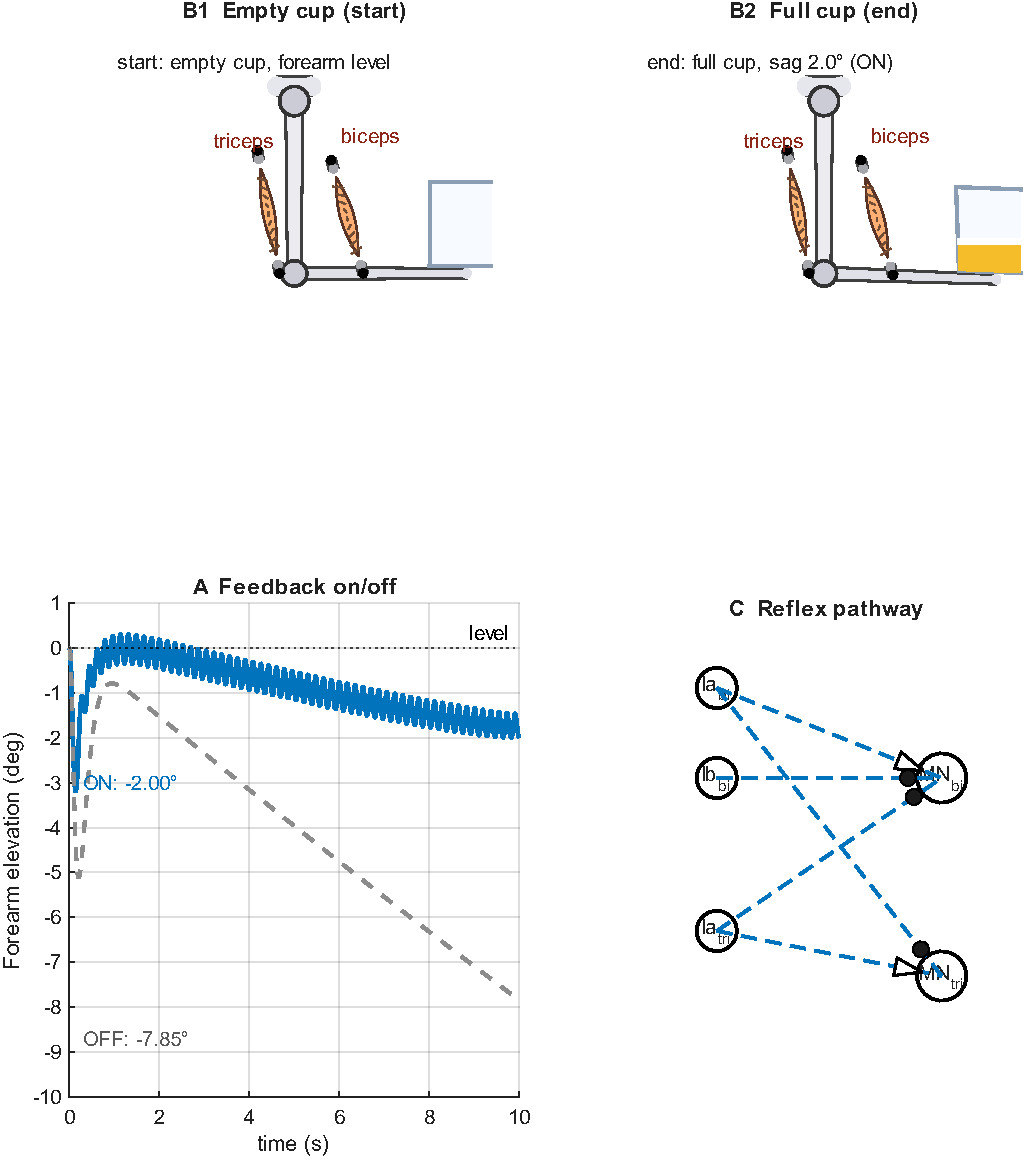
\includegraphics[width=\textwidth,height=0.80\textheight,keepaspectratio]{beverage_current_layout.pdf}
\caption{Loaded-arm demonstration: empty and loaded cup positions (A1, A2), feedback-on/off kinematics (B), and all six implemented feedback connections (C).}
\label{fig:sns_beverage_current}
\end{figure}

\FloatBarrier

\subsection{SOLIDWORKS-Derived Robot Assembly}\label{sec:sns_cad_methods}

I imported OpenSim-derived and SOLIDWORKS-derived mechanisms into Simscape Multibody. For the robot assembly, SNS-Simscape blocks connect the neural controller to BPA actuators using the force model, while joint and actuator measurements return through sensory blocks. This provides a graphical route from CAD geometry to a neuromechanical simulation. A separately assembled MuJoCo CAD model supplies additional integration and control tests (Appendix~\ref{sec:app_cad_supported_stance}).

A newer CAD-model comparison tests whether additional abductor control prevents the legs from crossing (Figure~\ref{fig:ah001_supported_control}). Under the same assistance settings, muscle-mediated separation feedback changed reversed ankle ordering from \qty{67}{\percent} of sampled states to zero. The model uses a layered SNS for timing together with an engineering force allocator. The allocator sets MN current targets for posture and separation, while the SNS supplies movement timing. This comparison demonstrates supported model integration and a separation-control effect. Appendix~\ref{sec:app_cad_supported_stance} gives the matched measures and foot-mount sensitivity.

\begin{figure}[p]
\centering
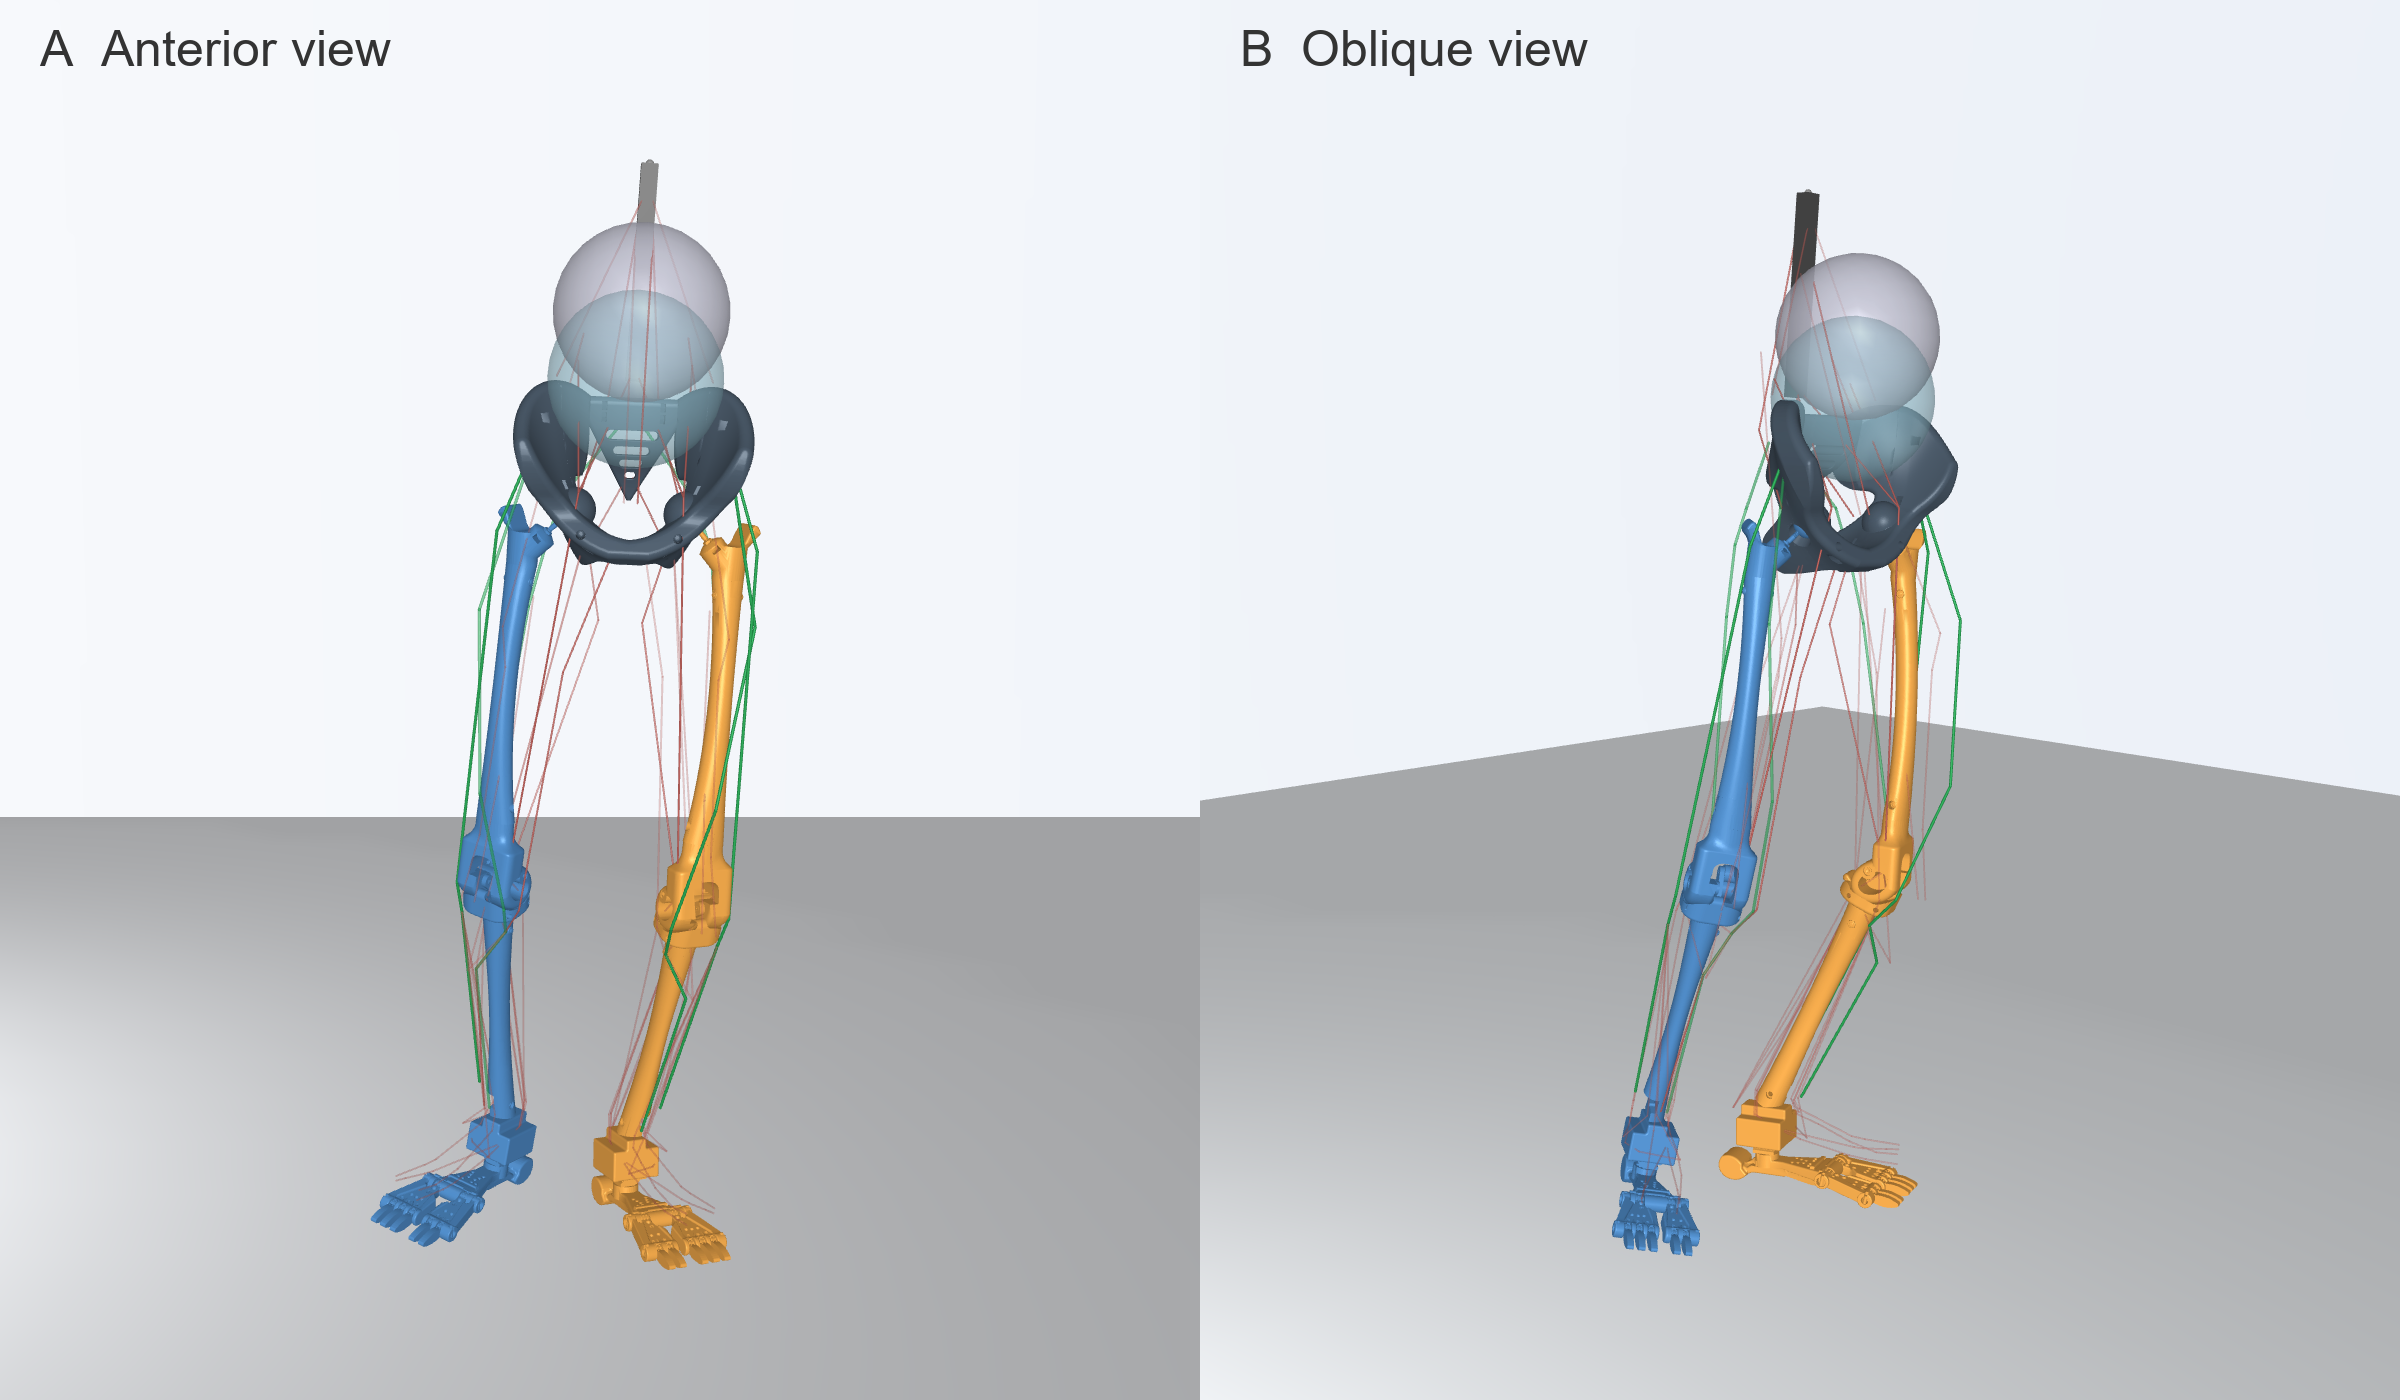
\includegraphics[width=\textwidth,height=0.55\textheight,keepaspectratio]{ah001_supported_control.png}
\caption[CAD-derived robot under supported hybrid control]{Anterior (A) and oblique (B) views of the same recorded CAD-model state. Right and left legs are blue and gold; selected hip-abducting routes are green. The \qty{75}{\kilogram} model uses 54 reference-tension actuators with hybrid neural and postural control. Vertical assistance supplies 80\% of body weight in this interval; lateral and angular assistance remain active. Attachments, the welded foot mount, and passive knee stops are provisional.}
\label{fig:ah001_supported_control}
\end{figure}

\FloatBarrier

\subsection{MuJoCo--Simulink Integration}\label{sec:sns_bridge_methods}

The MathWorks MuJoCo--Simulink bridge couples a block-programmed neural controller to a MuJoCo mechanical model. SNS-Simscape outputs supply actuator commands, and muscle length, velocity, force, and joint measurements return to the controller. A controller can therefore be edited graphically in Simulink and tested with MuJoCo mechanics. I implemented and tested the neural and actuator signal connections supplied through this bridge.

To test this connection, I paired the bridge with SNS-Simscape and compared single-muscle activation, different control rates, and sensor readback against a Python integration. Readback was bit-exact over the scored window. An exported neural network also drove all 92 actuator channels during a \qty{5}{\second} run without afferent return; a separate closed-loop reflex experiment exercised both commands and sensory measurements. These tests verify signal exchange through the interface. Under constant neural drive, one Simulink circuit realization reached a steady, nonoscillating state while its NumPy reference oscillated, showing why successful signal exchange must be followed by circuit-specific dynamical checks before transferring tuned parameters.

\subsection{Curriculum and Experiment Drivers}\label{sec:sns_curriculum_main}\label{sec:sns_repeatability_main}

The training workflow combines the four neural-training operations presented by \citet{hunt_inrc_2019} with my five-stage physical curriculum (Table~\ref{tab:sns_curriculum}). The neural operations establish intrinsic rhythm, tune its entrainment to expected afferent signals, fit feedforward motor activation, and refine that activation with sensory feedback. The physical stages then test the coupled model in deafferented air motion, afferented air motion, standing, supported ground stepping, and refinement with reduced assistance. A controller must be assessed at each physical stage rather than advancing because its neural activity alone appears rhythmic.

For the gain searches, I used a tree-structured Parzen estimator to propose parameter combinations from earlier evaluations. Each candidate is tested through simulation, and saved configurations allow a selected controller to be replayed before the next condition is introduced.

The experiment drivers then hold a selected controller fixed while changing sensory pathways, drive, mechanical support, or external perturbations. Finalists are also replayed under small parameter perturbations. Gait scoring requires detected cycles before a score is interpreted as movement quality; unsuccessful runs cannot be promoted by a reserved numerical failure value. The reference-library comparison tests transfer beyond the tuning reference. These procedures provide a repeatable way to identify where a controller works and which changes disrupt it, rather than making a single favorable trajectory the endpoint of tuning. Detailed scoring and configuration records are in Appendix~\ref{sec:sns_tuning_methods}.

A separate training implementation follows the four-step approach presented by \citet{hunt_inrc_2019}: select a CPG whose undriven period is approximately twice the desired locomotor period; fit afferent input connections using expected feedback to recover the target timing; fit CPG--PF outputs to motor-neuron activation peaks; and fit Ia and Ib feedback to refine the activation pattern. These parameter-training operations are distinct from the physical evaluation tasks in Table~\ref{tab:sns_curriculum}. With the Gait2392 human model, one trained configuration passed deafferented and afferented air-motion checks and assisted standing; these checks provide the starting configuration for training load-bearing steps.

\begin{table}[htbp]
\centering
\caption[Five-stage controller-tuning curriculum]{Five-stage controller-tuning curriculum. Each selected controller seeds the next stage. Air-stepping stages are suspended; ground stages retain mechanical support. The table defines the physical tasks and evaluation measures; it does not imply that every controller has passed every stage.}
\label{tab:sns_curriculum}
\small
\begingroup
\renewcommand{\arraystretch}{1.22}
\begin{tabularx}{\textwidth}{@{}c>{\raggedright\arraybackslash}p{0.24\textwidth}*{2}{>{\raggedright\arraybackslash}X}@{}}
\toprule
\textbf{Stage} & \textbf{Training task} & \textbf{Condition introduced} & \textbf{What is evaluated} \\
\midrule
1 & Deafferented air stepping & Legs suspended; sensory feedback disabled & Rhythm generation and swing depth \\
\addlinespace[6pt]
2 & Afferented air stepping & Heel, toe, and load feedback enabled & Rhythm and swing with sensory feedback \\
\addlinespace[6pt]
3 & Standing balance & Standing posture and push perturbations & Ability to maintain posture during a push \\
\addlinespace[6pt]
4 & Harness-supported ground stepping & Ground contact with measured external support & Alternating stance load, swing-foot unloading and clearance, forward progression, and joint kinematics \\
\addlinespace[6pt]
5 & Contact-driven ground walking & Contact-driven pathway variant & Joint kinematics against a human reference cycle \\
\addlinespace[6pt]
\bottomrule
\end{tabularx}
\endgroup
\end{table}

A separate W2L configuration reproduced its supported-stepping trajectory in four independent replays, and all twelve reruns with \qty{1}{\percent} parameter perturbations retained supported stepping. This demonstrates that a saved controller can be replayed and tested in its local parameter neighborhood. The repeatability tests and the pathway-removal panels use separately specified support settings; their event counts are therefore reported separately. Appendix~\ref{sec:app_supported_replays} retains the event counts, bilateral phase, displacement, speed, and support accounting.

The support protocol combines a constant weight-support term with position guidance, providing controllable loading conditions during training. These components can be reduced progressively as the controller adapts to greater stance loading.

\FloatBarrier

\subsection{Literature Circuits and Spiking Variants}\label{sec:sns_literature_methods}\label{sec:sns_literature_results}\label{sec:layer_stimulus_main}

The circuit diagrams in Chapter~\ref{ch:background} provide the reference architectures for these tests: the Rybak RG/PF hierarchy (Figure~\ref{fig:rybak_cpg_circuit}), the two-joint PF populations in the Shevtsova model (Figure~\ref{fig:shevtsova_spinal_circuit}), and the Deng sensory--motor organization (Figure~\ref{fig:deng_connectome}). The Di Russo reflex network and Shinohara bilateral network (Figures~\ref{fig:afferent_connectomes} and~\ref{fig:shinohara_connectome}) provide further comparisons for afferent routing and interleg coordination. The experiments here test selected implemented mechanisms from this literature.

Biarticular mechanics require explicit consideration when organizing the pattern-formation layer. \citet{deng_biarticular_2023} tested a suspended rat-hindlimb model and compared active, passive-only, and disabled biarticular muscles during perturbations. Their results motivate explicit multi-joint pattern-formation groups and perturbation tests when adapting controllers to the W2L and Gait2392 models.

Selected literature-derived circuits were tested with matched inputs and layer-specific stimuli before interpreting coupled motion. The reduced Rybak circuit was tested without mechanics; the Deng-derived circuit drove a suspended W2L model. Spiking variants retained a continuous motor-activation interface while changing the neural dynamics. Appendix~\ref{app:neuron_equations} gives their equations and calibration, and Appendix~\ref{sec:spiking_methods} gives the comparisons.

A complementary neural-only test distinguishes mechanisms that can produce a missing motor burst. In the reduced Rybak implementation, pattern-formation stimulation suppresses flexor motor output while the rhythm generator continues; rhythm-generator stimulation shifts the subsequent phase. Reproducing that distinction demonstrates the use of controlled interventions to test circuit organization before adding mechanical coupling (Appendix~\ref{sec:rybak_verification}).

A missing motor burst can arise from a disturbance of the rhythm generator or from suppression farther downstream. I applied stimuli separately to the RG, PF, and MN layers of a reduced Deng-derived circuit \citep{deng_neuromechanical_2019,nourse_sns_2023}. A resetting deletion suppresses expected motor activity and shifts the subsequent rhythm; a non-resetting deletion suppresses activity while preserving the original schedule. Matched baseline and stimulus runs distinguish the rhythm-generator clock from the motor output.

Stimuli lasting two baseline periods suppressed two expected flexor motor bursts at each layer. RG stimulation shifted both RG and motor timing by 0.211 cycles, whereas PF stimulation and direct MN inhibition preserved the original schedule. A separate \qty{1}{\second} PF stimulus shifted motor timing by 0.208 cycles while leaving the RG clock unchanged. The comparison separates motor-pattern timing from rhythm-generator resetting. The smaller-current sweep produced no observable deletions. Appendix~\ref{sec:app_layer_stimulus} gives the protocols and all stronger-current controls. A separate bilateral W2L test shows how brief hip-PF inhibition changes motor and joint responses while RG activity continues (Figure~\ref{fig:w2l108_pf_bilateral}).

\begin{samepage}
Spiking-neuron comparisons preserved a continuous motor-activation interface while changing rhythm timing and, in some runs, limb coordination (Appendix~\ref{app:simulation_verification}).\par
\end{samepage}


A public biarticular rat-hindlimb model was also imported for circuit inspection. It contains bilateral hindlimb mechanics, 120 neurons, sixteen muscles, and native RG, PF, and biarticular subnetworks (Figure~\ref{fig:rat_native_subnetworks}). This public precursor retains a fixed pelvis; it is distinct from the reduced fourteen-neuron test and from the final published 2023 implementation.
\begin{sidewaysfigure}[p]
\centering
\includegraphics[width=\textheight,height=0.87\textwidth,keepaspectratio]{DENG_RAT_NATIVE_SUBNETWORKS.pdf}
\caption[Imported biarticular hindlimb model and native subnetworks]{Imported public biarticular hindlimb precursor: model geometry and selected native hierarchy, rhythm-generation, hip pattern-formation, and biarticular coupling pages. Native neuron positions and internal connection routes are retained. BFP and RF identify biceps-femoris posterior and rectus-femoris pathways. The static model view shows geometry; it is separate from the W2L stepping experiments.}
\label{fig:rat_native_subnetworks}
\end{sidewaysfigure}

\subsection{Execution Speed and Actuator Implementations}\label{sec:sns_execution}

The accelerated workflow stores circuit topology and connection indices once, evaluates only existing synapses, reuses preallocated state and recording arrays, and compiles repeated neural, sensory, and muscle calculations with Numba where supported. Reference and accelerated implementations are compared under the same inputs, integration steps, and mechanical conditions before using the faster backend for training. Table~\ref{tab:sns_runtime} distinguishes complete coupled-loop timings from neural-only timings after warm-up. Loading, compilation, file output, and animation rendering are excluded.

\begin{table}[htbp]
\centering
\caption[Measured neural and coupled-model acceleration]{Execution times on easteregg2 after warm-up. The Gait2392 reference uses native SNS-Toolbox; W2L uses the same ported equations in Python. Neural-only rows exclude mechanical integration. The equation-kernel row compares a Di Russo-inspired Python implementation with its compiled Numba implementation.}
\label{tab:sns_runtime}
\small
\begin{tabularx}{\textwidth}{@{}Xrrrr@{}}
\toprule
Computation & Workload & Reference (s) & Fast (s) & Speedup \\
\midrule
\multicolumn{5}{@{}l}{Coupled MuJoCo models} \\
Gait2392 balance & 8 s & 122.120 & 13.253 & $9.21\times$ \\
W2L80 suspended & 4 s & 17.208 & 0.970 & $17.75\times$ \\
\addlinespace[5pt]
\multicolumn{5}{@{}l}{Neural calculations only} \\
SNS-Toolbox, 1,027 neurons & 500 updates & 24.534 & 0.245 & $100.17\times$ \\
Same benchmark, quiet repeat & 500 updates & 14.306 & 0.253 & $56.55\times$ \\
Python equation kernel & 1 update & $1.978\times10^{-3}$ & $3.385\times10^{-6}$ & $584.33\times$ \\
\bottomrule
\end{tabularx}
\end{table}

The 1,027-neuron benchmark accelerated fixed-conductance neural updates by 100.17 times, with a maximum voltage discrepancy of \qty{3.55e-15}{\milli\volt}. A quiet-machine repeat measured 56.55 times acceleration. The separately compiled Di Russo-inspired neural equations reached 584.33 times acceleration over their Python implementation. Mechanical integration, contact, and muscle calculations account for the smaller speedups of complete coupled simulations.

The saved Gait2392 positions, controls, center-of-mass, and neural arrays were identical between backends. The W2L comparison had a maximum force difference of \qty{7.94e-11}{\newton}. Its accelerated loop ran approximately 4.13 times faster than real time. The newer 108-neuron ground example advanced ten simulated seconds in \qty{4.265}{\second}, approximately 2.34 times real time. Matched whole-model AnimatLab and SNS-Simscape timings were not measured for these comparisons; their graphical construction and inspection roles complement headless training. Additional backend checks are retained in Appendix~\ref{app:simulation_verification}.

Actuator mechanics introduce a separate trade-off. The implementations include the converted biological-muscle models and the quasi-static BPA force calculation; a compliant-tendon prototype adds dynamic fiber and tendon equilibrium. In an isolated benchmark, 92 compliant muscle units advanced \qty{16}{\second} of simulated time in \qty{3.55}{\second} after compilation, approximately 4.51 times real time. The separately timed muscle bank therefore advances faster than real time. The prototype also includes fiber damping; separate joint-damping tests checked transient response. The additional equilibrium calculation increases cost relative to rigid-tendon actuation. These alternatives allow actuator fidelity and execution cost to be examined separately when selecting a model for controller training or eventual hardware control.

A separate BPA test interface combines the static Festo force surface with chamber-pressure dynamics and a synthetic hysteresis term based on filtered shortening and lengthening velocity. This history-dependent term provides a controlled actuator-model discrepancy for neural-compensation tests; identifying its parameters from dynamic BPA measurements is a direction for future research.

The integration culminates in the SOLIDWORKS-derived robot assembly coupled in SNS-Simscape to a synthetic neural controller and BPAs using my force model, with a virtual harness assisting standing. This example combines graphical neural construction, CAD mechanics, artificial-muscle forces, and sensory return in one model. It provides a starting point for studying the transition from supported posture to coordinated movement.

\section{Discussion: What the Tools Establish}\label{sec:sns_discussion}

The tools connect graphical neural construction, detailed mechanics, alternative actuator laws, and automated experiments. Matched neural traces establish implementation agreement, and command and sensor exchange through the bridge couples block-programmed controllers to MuJoCo models. The W2L comparison identifies a sensory-feedback contribution to bilateral contact coordination, while the loaded-arm example demonstrates a corrective response in the coupled neural and actuator blocks.

These simulations provide a platform for investigating neural coordination with experimentally characterized BPA forces. Motor-neuron outputs are converted to actuator excitation or pressure commands, and sensory feedback allows the controller to respond to the resulting movement and loading. Future researchers can extend this simulated BPA control through improved dynamic characterization and closed-loop hardware experiments, including pressure response, loading-dependent behavior, and neural compensation for actuator-model errors. Chapter~\ref{ch:overall} connects these opportunities with the actuator characterization, torque models, SADb, and robot design.
